\section{Introduction}\hfill

% The Large Hadron Collider~\cite{LHC}, LHC, is the largest and highest energy particle collider ever constructed by humankind. Using superconducting magnets, protons are accelerated around a 27km ring and collide in designated interaction points at a center of mass energy of 14TeV. The proton-proton interactions produce heavy particles which decay into a higher multiplicity of lighter particles. This decay chain results in a cascading effect which creates a shower of particles observed by the detector. If particles originate from a common heavy ancestor, they often form collimated streams of lighter particles in a tight cone, which are referred to as jets.

At the Large Hadron Collider, LHC, the ATLAS and CMS experiments look at the interactions of elementary particles to better understand the fundamental structure of nature. These studies are performed by colliding groups of protons, or bunches, at extremely high energies. At such high energy, each collision leads to the production of hundreds of particles which are registered by the ATLAS and CMS detectors. The information recorded by the detectors are referred to as an \emph{event}. Since each bunch contains $10^{11}$ protons, each event contains information from multiple proton-proton interactions. The average number of interactions per bunch crossing recorded in an event is referred to as $\left\langle \mu \right\rangle$. The events selected for recording are chosen in such a way that at least one of these interactions is a \emph{hard scatter}, considered as \emph{signal}, which contains highly energetic particles that are of interest to physics. Other interactions recorded in the same event are called \emph{pileup}, considered as \emph{background}, which contaminates the signal.

\begin{figure}[ht]
\centering
  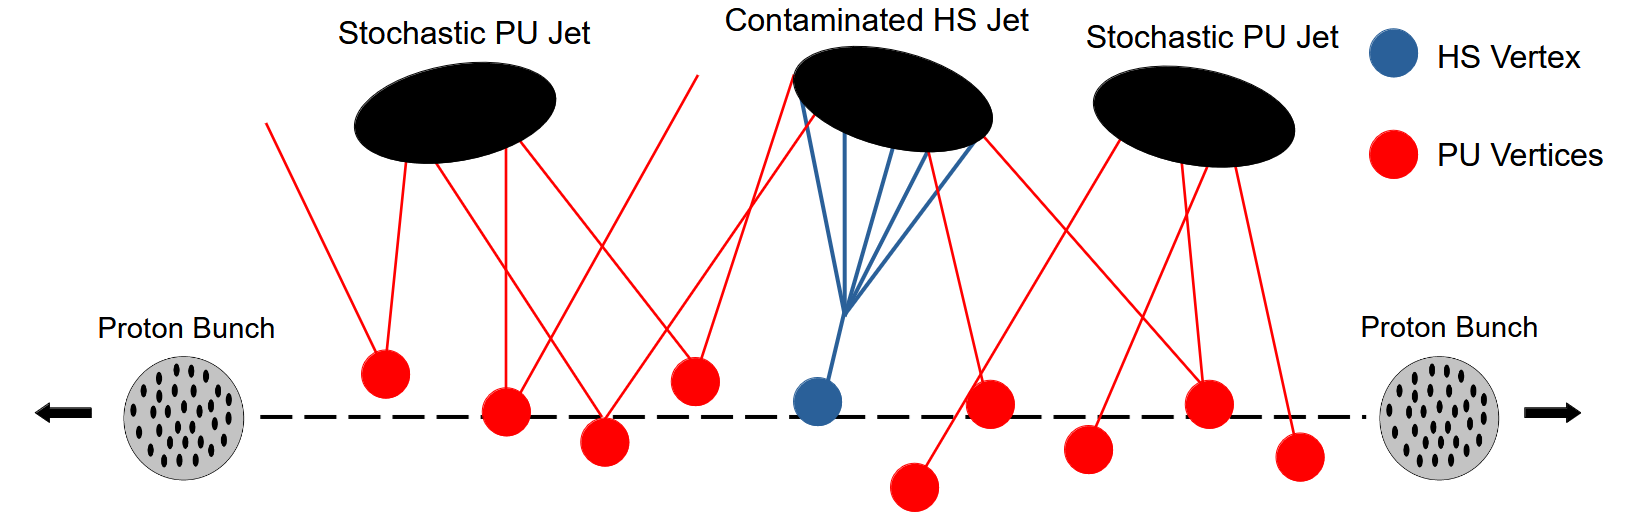
\includegraphics[width=1\linewidth]{Pileup_Graphic.png} 
  \caption{The interactions from crossing proton bunches in a single event. Hard scatter, HS, interaction originates from the primary vertex while other interactions, PU, originate from pileup vertices. The jets that originate from the HS vertex form a correlated set, while the jets from PU are stochastic in nature and do not have correlations.}
\label{fig:PileupJets}
\end{figure}

Our research focuses on physics processes where particles form streams that can be clustered into tightly knit cones called \emph{jets}, which can originate from both hard scatter and pileup collisions. Throughout this article, we refer to particles as \emph{tracks}, and the collision points from which the tracks originate as \emph{vertices}. In a real experiment, jets are measured and identified using information from many subdetector systems, but to simplify the problem, in this paper we treat jets purely as sets of tracks. While jets containing tracks due to hard scatter are of actual physics interest, there are many jets originating from the pileup interactions (Figure~\ref{fig:PileupJets}). Pileup mitigation techniques employed so far typically follow a two-step approach: (i) a binary classification task to identify jets as hard scatter or pileup~\cite{ATLAS-CONF-2014-018}, and (ii) application of energy and mass corrections to jets identified as hard scatter through algorithms such as Charged Hadron Subtraction~\cite{CHS}.

%\arun{Should we remove this last sentence as we detail about this in the next paragraph? Instead, shall we give a sentence motivation for jet level binary classification problem?} The main purpose of this study is (1) to identify the jets from hard scatter and pileup and (2) to measure the level of contamination of hard scatter jets from pileup tracks.

%At the Large Hadron Collider (LHC)~\cite{LHC}, physicists study to better understand phenomena of the universe related to the fundamental forces of nature. These proton-proton collisions produce elementary particles that are irreducible quanta of energy.
%described by the Standard Model of Particle Physics. 
%Due to the subatomic size of protons, the mean number of interactions per bunch crossing, $\left\langle \mu \right\rangle$, is very small. Only one of these collisions interacts via a strong head-on collision that produces deep inelastic scattering called \emph{hard scatter} or \emph{signal}, while other weaker interactions are called \emph{pileup} or \emph{background}. 
%In addition to hard scatter, there exists many other soft collisions arising from weaker interactions which are called \emph{pileup}. 

%Each of these collisions, in turn, produces heavy particles which decay into lighter particles in a cascading effect. Streams of such decayed particles are called \emph{jets}, which can be clustered to form a tightly knit cone containing charged particles, called \emph{tracks}. All these collisions are recorded as \emph{events}, usually at a rate of every 25 nanoseconds, containing a variable number of jets and a variable number of tracks in each jet. It is important to note that jets originating from hard scatter processes share underlying physics and thus can be correlated with other jets in the hard scatter process. Such a correlation is not feasible for pileup jets due to their stochastic nature, as given in Figure~\ref{fig:PileupJets}.

%The Large Hadron Collider~\cite{LHC}, LHC, is the largest and highest energy particle collider ever constructed by humankind. Using superconducting magnets, protons are accelerated around a 27km ring and collide in designated interaction points at a center of mass energy of 14TeV. This decay chain results in a cascading effect which creates a shower of particles observed by the detector.
%The proton-proton interactions that happen in colliders like Large Hadron Collider~\cite{LHC} produce heavy particles which decay into a higher multiplicity of lighter particles in a cascading effect. 
%\textcolor{red}{We need to simplify these two sentences.} Streams of such lighter particles originating from a common ancestor are called \emph{jets}, they often form collimated streams of lighter particles in a tight cone, which are referred to as jets.

%General purpose detectors at the LHC consist of two main components: a tracker and a calorimeter. The tracker uses silicon dots and strips to measure the position and momentum of each particle that passes through it. Particles that are reconstructed using the tracker are referred to as tracks. The calorimeter uses dense material, such as lead, to absorb and record the energy of particles. A stream of collimated particles that deposits energy into the calorimeter is reconstructed as a jet.

%Due to the very small interaction cross-section of proton-proton collisions, bunches of 100 billion protons are collided at the same time to increase the rate of interaction. On average, there will be zero or one collisions that interact "head on" producing deep inelastic scattering. This type of interaction is called the Hard Scatter, HS, process. However, in the current LHC configuration, there exists, on average, an additional 60 other interactions from various protons in the bunch crossing that are physically piled up on top of the hard scatter interaction. These additional interactions are referred to as Pileup, PU, processes.



%Pileup interactions are considered as contamination because of their ample quantities compared to signal processes. It is important to identify and mitigate pileup from each collision events to increase sensitivity of signal processes and assist physicists to discover new particles. 

%Machine learning and AI methods have been introduced in recent years to help physicists analyze data at the LHC. Machine learning has been applied to several sub-problems in High Energy Physics~\cite{he2023high,Larkoski_2020}, such as jet flavor tagging~\cite{ParticleNet}, top tagging~\cite{Barman_2024}, generative event modeling~\cite{kansal2021particle}, and anomaly detection. While machine learning techniques have been applied to analyze pileup~\cite{komiske2017pileup,ABCNet}, methods to analyze \emph{PileUp} at large $\left\langle \mu \right\rangle$ values have been mostly overlooked in the existing works. Although there is growing interest in this domain due to upcoming LHC upgrades, existing methods assume (i) only low pileup events, and (ii) pileup identification as a binary classification problem. As LHC prepares to upgrade to the High-Luminosity (HL)LHC~\cite{HLLHC}, with $\left\langle \mu \right\rangle = 200$, it brings exponentially higher number of pileup particles per event.

The LHC prepares to upgrade to the High-Luminosity phase, HL-LHC, where $\left\langle \mu \right\rangle$ will increase from 60 to 200. This upgrade will dramatically increase the number of pileup particles in each event, which will increase the statistics of rare hard scatter processes. However, in order to maximize the discovery potential of the HL-LHC, there is a need to mitigate high pileup conditions: in particular, to quantify the energy and momentum contributions from pileup to hard scatter jets. Existing methods have focused on investigating pileup at $\left<\mu\right>$ values below 60 ~\cite{ATLAS-CONF-2014-018}, but as $\left<\mu\right>$ approaches 200, the high pileup conditions degrade the quality of hard scatter jets to the point that binary classification is no longer suitable. The large pileup background shifts the problem to a continuous regression task which, in  turn, performs the simultaneous tasks of identification, energy correction, and mass correction of hard scatter jets.

Machine learning methods have become widespread in High Energy Physics, HEP, ~\cite{he2023high,Larkoski_2020} assisting with pileup mitigation~\cite{komiske2017pileup}, jet tagging~\cite{ParticleNet}, top tagging~\cite{Barman_2024}, event modeling~\cite{kansal2021particle} and searches for new physics using anomaly detection~\cite{duarte2024novelmachinelearningapplications} and other AI methods. The ATLAS experiment is using the JVT kNN algorithm~\cite{ATLAS-CONF-2014-018} which relies on constructing high level variables using track and jet features to perform binary classification on a per jet basis.  However, this method fails to incorporate correlations between jets and tracks at the event level. There have been attempts to introduce correlations between tracks and jets using graph neural networks~\cite{ParticleNet,ABCNet}, however, it has been shown~\cite{qu2022particle} that attention neural networks scale more efficiently which is a requirement for high pileup conditions.

This work proposes an attention-based neural network, \myname{}, to mitigate pileup by performing the simultaneous identification, energy correction, and mass correction of hard scatter jets. \myname{} uses self and cross attention to capture all possible correlations between jets and tracks within an entire event while maintaining good performance when scaling to high pileup conditions. \myname{} also outperforms benchmarks against existing methods in our experiments, and increases the discovery potential of the HL-LHC through a practical example of a physics analysis.

%\textcolor{violet}{In this work, we present the following contributions:
%\begin{enumerate}
%    \item We propose a first-of-its-kind pileup prediction modeled as a regression problem.
%    \item We propose cross-attention based neural network architecture that utilizes jets and tracks information for pileup fraction detection.
%    \item We show with extensive analysis that the proposed method outperforms the baseline approaches.
%    \item We also show that the predictions from the proposed approach also assist with physics processes.
%\end{enumerate}}


%\arun{I think there was a few sentences approximately how many millions/billions of collisions per proton bunch. That was interesting and would look good if we have it in one sentence in next paragraph.}

 
 %\luke{In low pileup conditions, the data is sparse such that jets can be easily binary classified as hard scatter or pileup jets. There could be a few pileup tracks entering a hard scatter jet, which can be corrected using Charged Hadron Subtraction~\cite{CHS}, but the overall mass and energy of the hard scatter jet are seemingly unaffected. This becomes challenging with the upcoming upgrades to LHC which introduces several noisy pileup tracks into hard scatter jets and eventually altering core properties of hard scatter jets.}


%\luke{In low pileup conditions, pileup is sparse enough such that jets tend to be binary classified as hard scatter or pileup jets as shown in figure \ref{fig:PileupJets}. There could exist a few tracks entering a hard scatter jet, which can be corrected using Charged Hadron Subtraction~\cite{CHS}, but the overall mass and energy of the hard scatter jet are seemingly unaffected. However if pileup increases, there exists a critical point in $\left\langle \mu \right\rangle$ where there is such a large pileup background that the mass and energy of hard scatter jets are significantly affected.}
%This critical point becomes more daunting as the LHC prepares to upgrade to the High-Luminosity (HL)LHC~\cite{HLLHC}. The HL-LHC will bring in much more data for hard scatter collisions at the cost of many more pileup collisions.

%\luke{The existing algorithms developed for pileup mitigation using binary classification at low pileup conditions for the LHC will start to struggle as pileup is increased for the HL-LHC. Therefore at high pileup conditions, future algorithms must consider pileup as continuous regression problem to determine by what fraction the \emp{hard scatter} jet's mass and energy has been affected by \emp{pileup}. In this paper we propose a model that attempts to solve the problem of pileup by directly predicting energy and mass fractions of each jet using transformer encoders using self-attention and cross-attention to learn enriched representations of jets using all possible correlations between jets and tracks within the context of an event.}

% \arun{Explain why it is necessary to identify pileup jets for physics processes.} \luke{Processes that lead to new physics, considered as signal, occur through \emph{hard scatter} interactions. All other interactions are considered \emp{pileup} and are a source of background which contaminates the signal. Therefore, the identification and suppression of the \emp{pileup} background is crucial to increase the sensitivity to signal of the \emp{hard scatter} processes. Pileup mitigation helps physicists to probe new physics and discover new particles by reducing the pileup background.}

%An event is defined as data recorded from a single bunch crossing which occur every 25 nanoseconds. Each event contains variable length set of jets. Each jet contains a variable length set of tracks. The hard scatter jets that originate from the same underlying physics process will be correlated with each other. On the other hand, pileup jets are formed due to stochastic nature and are not correlated to other jets in the event. Attention neural networks are capable of learning correlations between jets and allow for a context window of an entire event.

% \begin{figure}[h]
%   \centering
%   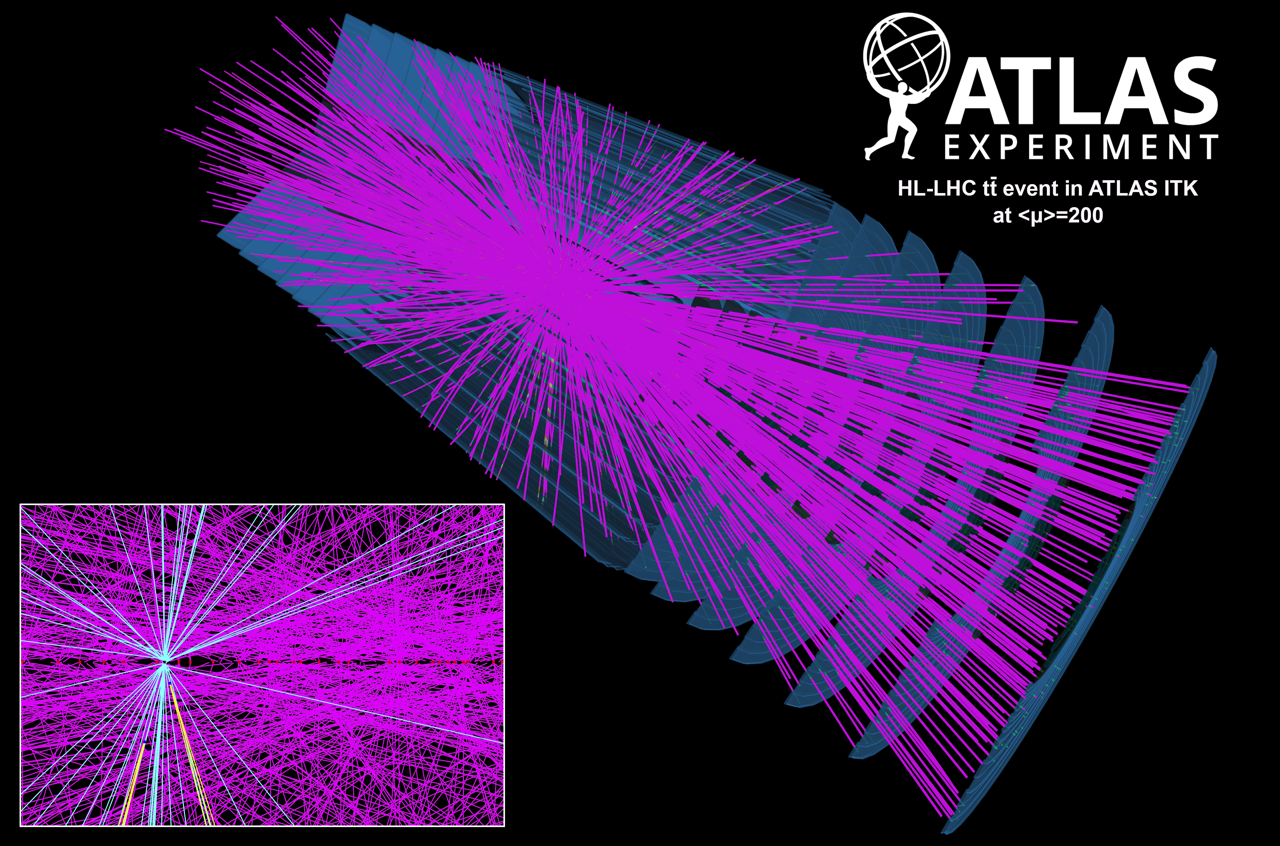
\includegraphics[width=0.75\linewidth]{HL-LHC-tt}
%   \label{fig:vertexing}
%   \caption{In the HL-LHC configuration, the Hard Scatter process (light blue) begins to be dominated by PileUp (purple). Note: https://atlas.cern/updates/news/scientific-potential-high-luminosity-lhc}
% \end{figure}

%In order to increase the amount of data collected, the LHC has plans to plans to increase the mean number of collisions, $\left<\mu\right>$, for what is called the High-Luminosity (HL)LHC~\cite{HLLHC}. The HL-LHC will increase the mean number of interactions up to $\left<\mu\right>=200$ to collect more data and increase statistics. This change in configuration of the LHC will bring much more pileup begins to dramatically blur the concept of a HS and PU jet. What was a binary classification task at low pileup conditions becomes a continuous regression task at high pileup conditions. This is due to the fact that there are so many pileup particles crammed into the $4\pi$ solid angle coverage of the detector, that nearly all hard scatter jets have a significant contribution to their mass and energy from pileup. 

%This motivates that jets should not be considered as binary HS or PU, but instead jets should have a continuous energy and mass corrections that are be applied to correct for pileup effects. In this paper, we propose an improvement to pileup mitigation at the HL-LHC using Multi-Head Attention and Transformer Encoder stacks~\cite{Attention} to perform a continuous regression task on jets in the context of an entire event. \\
